\chapter{Modelagem do Sistema}
\noindent
Este capítulo tem o objetivo de abordar a modelagem proposta para o sistema. Vale destacar que o sistema se propõe a não somente realizar o reconhecimento facial, como também permitir o armazenamento persistente das faltas apuradas, permitir a correção de eventuais erros de apuração e possuir mecanismos de consultas das faltas. O escopo do projeto abrange a apuração e o registro das faltas, sem incluir, portanto, a apuração de pontos perdidos.

\section{Levantamento de requisitos}
\noindent
O levantamento de requisitos é uma importante atividade para se entender o problema. Segundo \citep{bezerra}, essa etapa tem a finalidade de que desenvolvedores e usuários compartilhem da mesma visão do problema a ser solucionado. Buscou-se realizar uma série de procedimentos com a finalidade de levantar os requisitos funcionais e não-funcionais aqui expostos. Dentre as técnicas adotadas merecem destaque a análise de documentos, \textit{Brainstorming} e entrevistas informais.

\subsection{Requisitos Funcionais} 

Segundo \citep{bezerra} esse tipo de requisito está ligado às funcionalidades do sistema.  A seguir apresenta-se o resultado desse levantamento.

\begin{itemize}
\item RF01 - Apurar falta: O sistema deve apurar as faltas de um determinado tempo de aula em uma data, disciplina, para uma turma, usando o reconhecimento facial em uma fotografia da turma. As fotos devem ser tiradas por um dispositivo móvel com câmera ou selecionadas de sua galeria. Deve-se reconhecer várias faces em uma mesma fotografia, isso é, a fotografia é da turma e não individual. O professor deve poder enviar uma ou mais fotografias em um único tempo de aula, em operações de envio distintas. Assim ao enviar uma fotografia, e verificar que nem todos os alunos presentes receberam a presença, ele poderia enviar uma fotografia em adição à apuração anterior. Isso também ajuda, para os casos em que a turma não pode ser enquadrada em uma única fotografia. As informações referentes a data, isso é, dia, mês e ano devem ser extraídas do servidor; 

\item RF02 - Verificar lista de presença : Um aluno, coordenador ou professor deve ser capaz de  exibir a lista de presença referente a um determinado tempo de aula, de um determinado dia para uma turma específica; 
\item RF03 - Editar lista de presença : O professor deve ser capaz de alterar as faltas de um tempo de aula, isso permite que ele corrija eventuais erros na apuração de faltas que usou o reconhecimento facial; e 
\item RF04 - Armazenar fotografia : Deve-se armazenar a fotografia com sua apuração no servidor, em uma pasta específica para isso, permitindo uma eventual auditoria.
\end{itemize}

\subsection{Requisitos Não-Funcionais}
Tratam sobre características do sistema, \citep{bezerra} elenca alguns tipos como confiabilidade, desempenho, portabilidade, segurança e usabilidade. A seguir apresenta-se os requisitos não-funcionais levantados.

\begin{itemize}
%\item RN01 - O índice de erro no reconhecimento facial deve ser inferior a 50\%. Considera-se como erro, apenas os casos em que a face da pessoa X é reconhecida como sendo da pessoa Y. A classificação como desconhecida não caracteriza um erro de reconhecimento;

\item RN01 - O Sistema deve apresentar interface com o usuário “Professor” compatível com o  sistema Android; 

\item RN02 - O banco de dados, no qual se fará o armazenamento persistente, deve ser PostgreSQL;

\item RN03 - As tarefas de captura de foto, reconhecimento facial e armazenamento de registros devem ser feitas em módulos distintos; e

\item RN04 - Um professor deve ser capaz de utilizar o sistema após um treinamento de 15 minutos.

\end{itemize}


\section{Casos de uso}
\noindent
Segundo \citep{bezerra}, o modelo de casos de uso  consiste em um refinamento dos requisitos funcionais. Acrescenta que os casos de uso tratam sobre funcionalidades externas do sistema, assim não se abordam mecanismos internos. Assim, com base nos requisitos funcionais apresentados no tópico 3.1.1, tem-se a figura \ref{fig:figura03} que traz o diagrama de casos de uso. Vale destacar que o RF04 foi incorporado ao RF01 gerando um único caso de uso, isso se explica pois o armazenamento da imagem só ocorre posteriormente à apuração das faltas. Os atores \textbf{professor} e \textbf{usuário} são apresentados utilizando-se  o relacionamento de generalização entre atores. Além disso usuário também comporta os alunos e os coordenadores. 

%altearar figura
\begin{figure}[!ht]
	\centering
	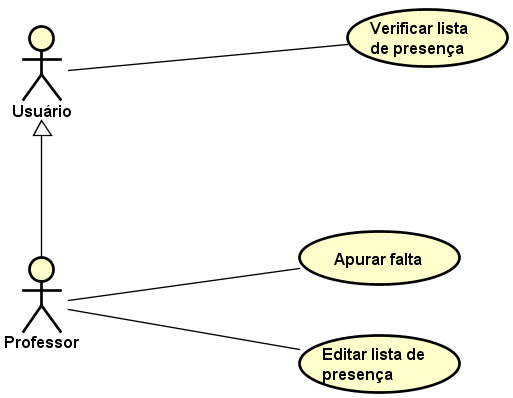
\includegraphics[width=0.8\textwidth]{dcu.png}   
	\caption{Diagrama de casos de uso}
	\label{fig:figura03}
\end{figure}
Nas subseções seguintes é feito o detalhamento dos casos de uso \textbf{apurar falta}, \textbf{editar lista de presença}, \textbf{verificar lista de presença}.


\subsection{Apurar Falta} 
\noindent
Identificador e nome: UC-01. Apurar falta.

Sumário: O ator utiliza esta função para apurar as faltas de um tempo de aula específico, através de uma fotografia da turma.

Ator Principal: Professor.

Pré-condição: O ator começa um tempo de aula e inicia o aplicativo Android Tchau Papeletas.

Fluxo Principal:

1- O ator solicita a função apurar faltas.

2- O sistema apresenta os campos código e tempo de aula para preenchimento e seleção, respectivamente. Além do campo para a fotografia.

3- O ator preenche com o código, formado pelo nome da turma + '.' + nome da matéria, e seleciona o tempo de aula.

4- O ator seleciona uma imagem previamente existente  ou abre a câmera do dispositivo e fotografa a turma.

5- O ator clica em enviar.

6- O sistema acusa \textit{upload} realizado com sucesso.

Pós-condição: A apuração de faltas daquele tempo de aula foi realizada e registrada no banco de dados, uma imagem com as faces identificadas foi salva no servidor.


\subsection{Editar Lista de presença} 
\noindent
Identificador e nome: UC-02. Editar Lista de presença.


Sumário: O ator utiliza esta função para alterar as faltas apuradas no UC-01. Permitindo assim, correções na apuração pelo reconhecimento facial.

Ator Principal: Professor

Pré-condição: Uma apuração utilizando o reconhecimento facial já foi realizada para aquele tempo de aula.

Fluxo Principal:

1- O ator solicita a função editar lista de presença.

2- O sistema apresenta os campos código e tempo de aula, além de dia, mês e ano.

3- O ator preenche os campo nome da turma, nome da matéria, tempo de aula e a data, formada por dia, mês e ano.

4- O sistema exibe a papeleta de faltas preenchida, com as faltas apuradas pelo UC-01. Essa papeleta contém em seu cabeçalho a disciplina, o tempo de aula, data (dia, mês e ano) e turma. Em seu corpo, o código do aluno (matrícula), o nome do aluno e a presença ou ausência do aluno. Esse último campo é editável. Na parte inferior um botão de confirmar alterações.

5- O ator realiza as alterações de presença que julgar ser necessário. Ao final, pressiona o botão  de confirmar alterações.

6- O sistema exibe uma mensagem de alerta, pedindo uma nova confirmação. 

7- O ator confirma a operação.

8- O sistema acusa atualização realizada com sucesso.

Pós-condição: A apuração de faltas daquele tempo de aula foi alterada e registrada no banco de dados.


\subsection{Verificar Lista de Presença} 
\noindent
Identificador e nome: UC-03. Verificar Lista de Presença.

Sumário: O ator utiliza esta função com a finalidade de verificar as faltas de um tempo de aula específico. Seria similar a observar a papeleta de faltas preenchida.

Ator Principal: Aluno, Coordenador  e Professor

Pré-condição: Uma apuração utilizando o reconhecimento facial já foi realizada para aquele tempo de aula.

Fluxo Principal:

1- O ator solicita a função verificar lista de presença.

2- O sistema apresenta os campos código e tempo de aula, além de dia, mês e ano.

3- O ator preenche os campo nome da turma, nome da matéria, tempo de aula e a data, formada por dia, mês e ano.

4- O sistema exibe a papeleta de faltas preenchida, com as faltas apuradas pelo UC-01 e possivelmente alteradas pelo UC-02 . Essa papeleta contém em seu cabeçalho a disciplina, o tempo de aula, data (dia, mês e ano) e turma. Em seu corpo, o código do aluno (matrícula), o nome do aluno e a presença ou ausência do aluno.

Pós-condição: O sistema permanece inalterado.




\section{Conceito Geral do Sistema}
\noindent
A partir das etapas anteriores, pode-se depreender o conceito geral do sistema e como ele será trabalhado. Segundo \citep{engenhariasoftware} a engenharia de \textit{software} tem como objetivo principal a entrega do \textit{software} em tempo hábil, com alta qualidade e que atenda aquilo que lhe foi requisitado. Para atender esse objetivo, \citep{engenhariasoftware} elenca uma série de princípios, dentre os quais, se destaca o conhecido princípio dividir para conquistar, que como o nome sugere se trata de subdividir o problema em partes menores. Posteriormente, os mencionados autores depreendem desse princípio um outro, que é o de construir \textit{softwares}  apresentando o que chamam de modularidade efetiva. Sobre isso, afirmam que: "cada módulo deve se concentrar exclusivamente em um aspecto bem restrito do sistema – deve ser coeso em sua função e/ou apresentar conteúdo bem preciso"\ \cite[p. 109]{engenhariasoftware}.
% citar página 109 do engenhariasoftware

A modularidade permite que um módulo seja substituído por outro, sem que se tenha de alterar o sistema como um todo, além disso facilita a manutenção, uma vez que cada módulo tem um propósito bem definido. O sistema se dividirá em 3 módulos, a saber:

\begin{itemize}
\item \textit{Módulo Servidor:} esse é o responsável por receber a fotografia tirada da turma, assim como os dados como turma, dia, hora e matéria. Ele deverá detectar as faces na fotografia e depois, utilizando o algoritmo escolhido, identificar cada uma delas. Para cada face reconhecida deve-se atribuir a presença, a qual será enviada para o armazenamento persistente;
\item \textit{Módulo Mobile:} ele permitirá que o professor fotografe a turma, insira os dados mencionados acima, e encaminhe para o servidor, oferecendo ao professor uma interface amigável. Além disso, ele permitirá que o professor visualize a papeleta digital após a apuração e a corrija, se for o caso. Para tal, será projetado para o sistema \textit{Android}; e
\item \textit{Módulo BD:} é onde se dará o armazenamento persistente das informações. Ele terá as informações sobre os alunos, como nome, turma, matrícula, disciplinas daquela turma, e é claro a presença/falta no tempo de aula.
\end{itemize}

%A figura \ref{fig:figura04} mostra o funcionamento do sistema descrito acima:

%\begin{figure}[!ht]
%	\centering
%	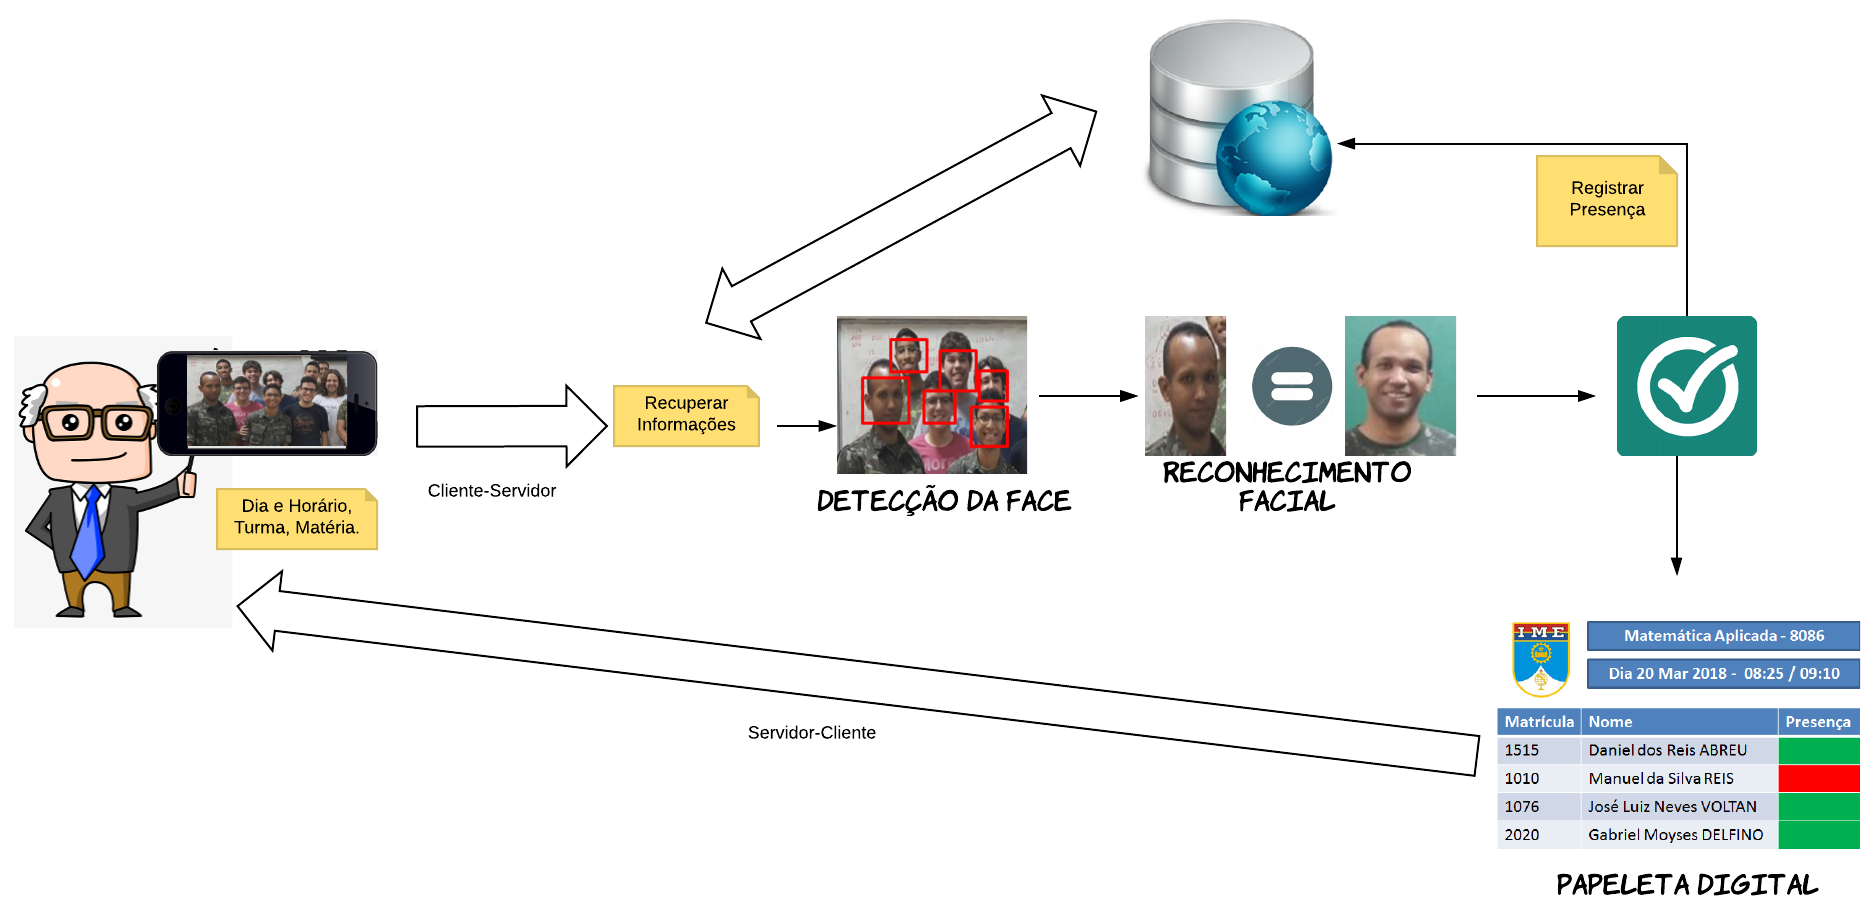
\includegraphics[width=1\textwidth]{esquema.png}   
%	\caption{Modelo de funcionamento geral do sistema}
%	\label{fig:figura04}
%\end{figure}

Pode-se ainda detalhar as atividades envolvidas no processo de reconhecimento facial através de um diagrama de atividades, conforme a figura \ref{fig:figura05}. 

\begin{figure}[!ht]
	\centering
	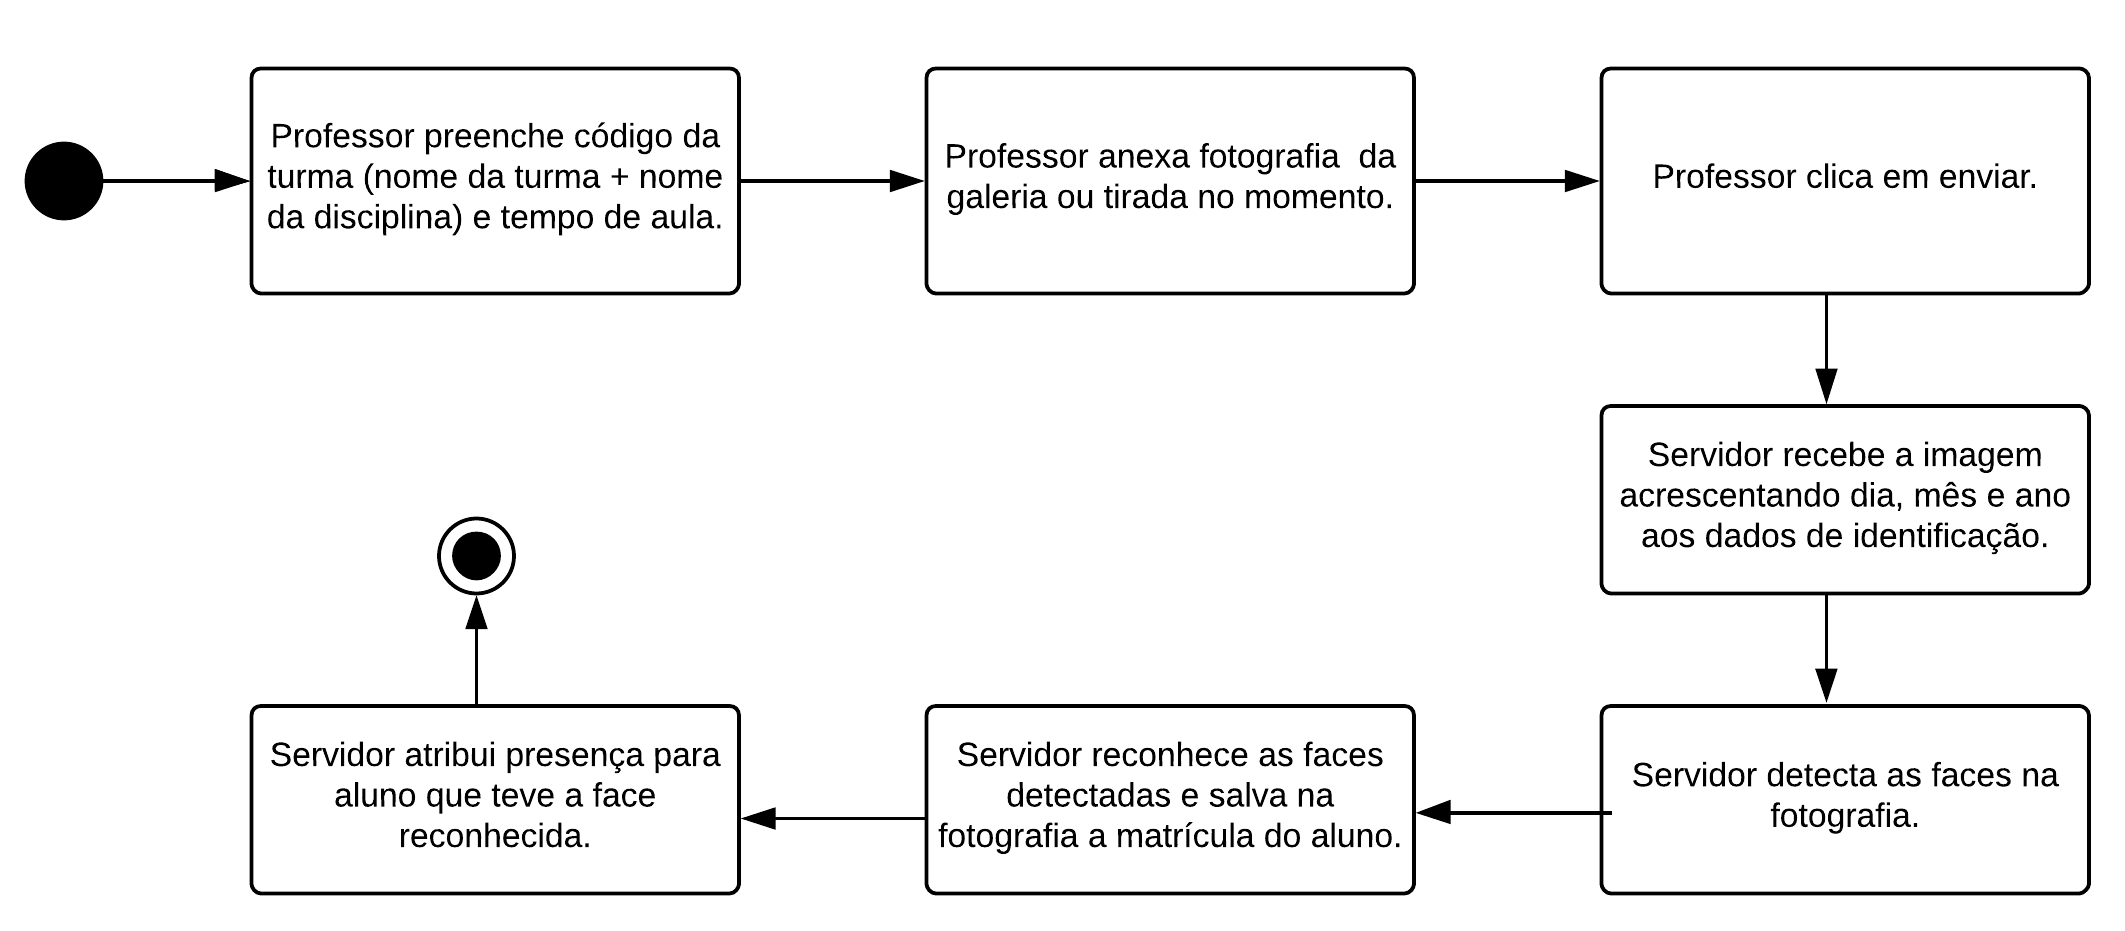
\includegraphics[width=1\textwidth]{diagativigeral.png}   
	\caption{Diagrama de atividades para o reconhecimento facial}
	\label{fig:figura05}
\end{figure}

%Os módulos devem se comunicar de maneira eficiente, permitindo que o sistema atinja seu objetivo.

